%!TEX root = ../dissertation.tex
\chapter{Implementation}

%\begin{figure}
%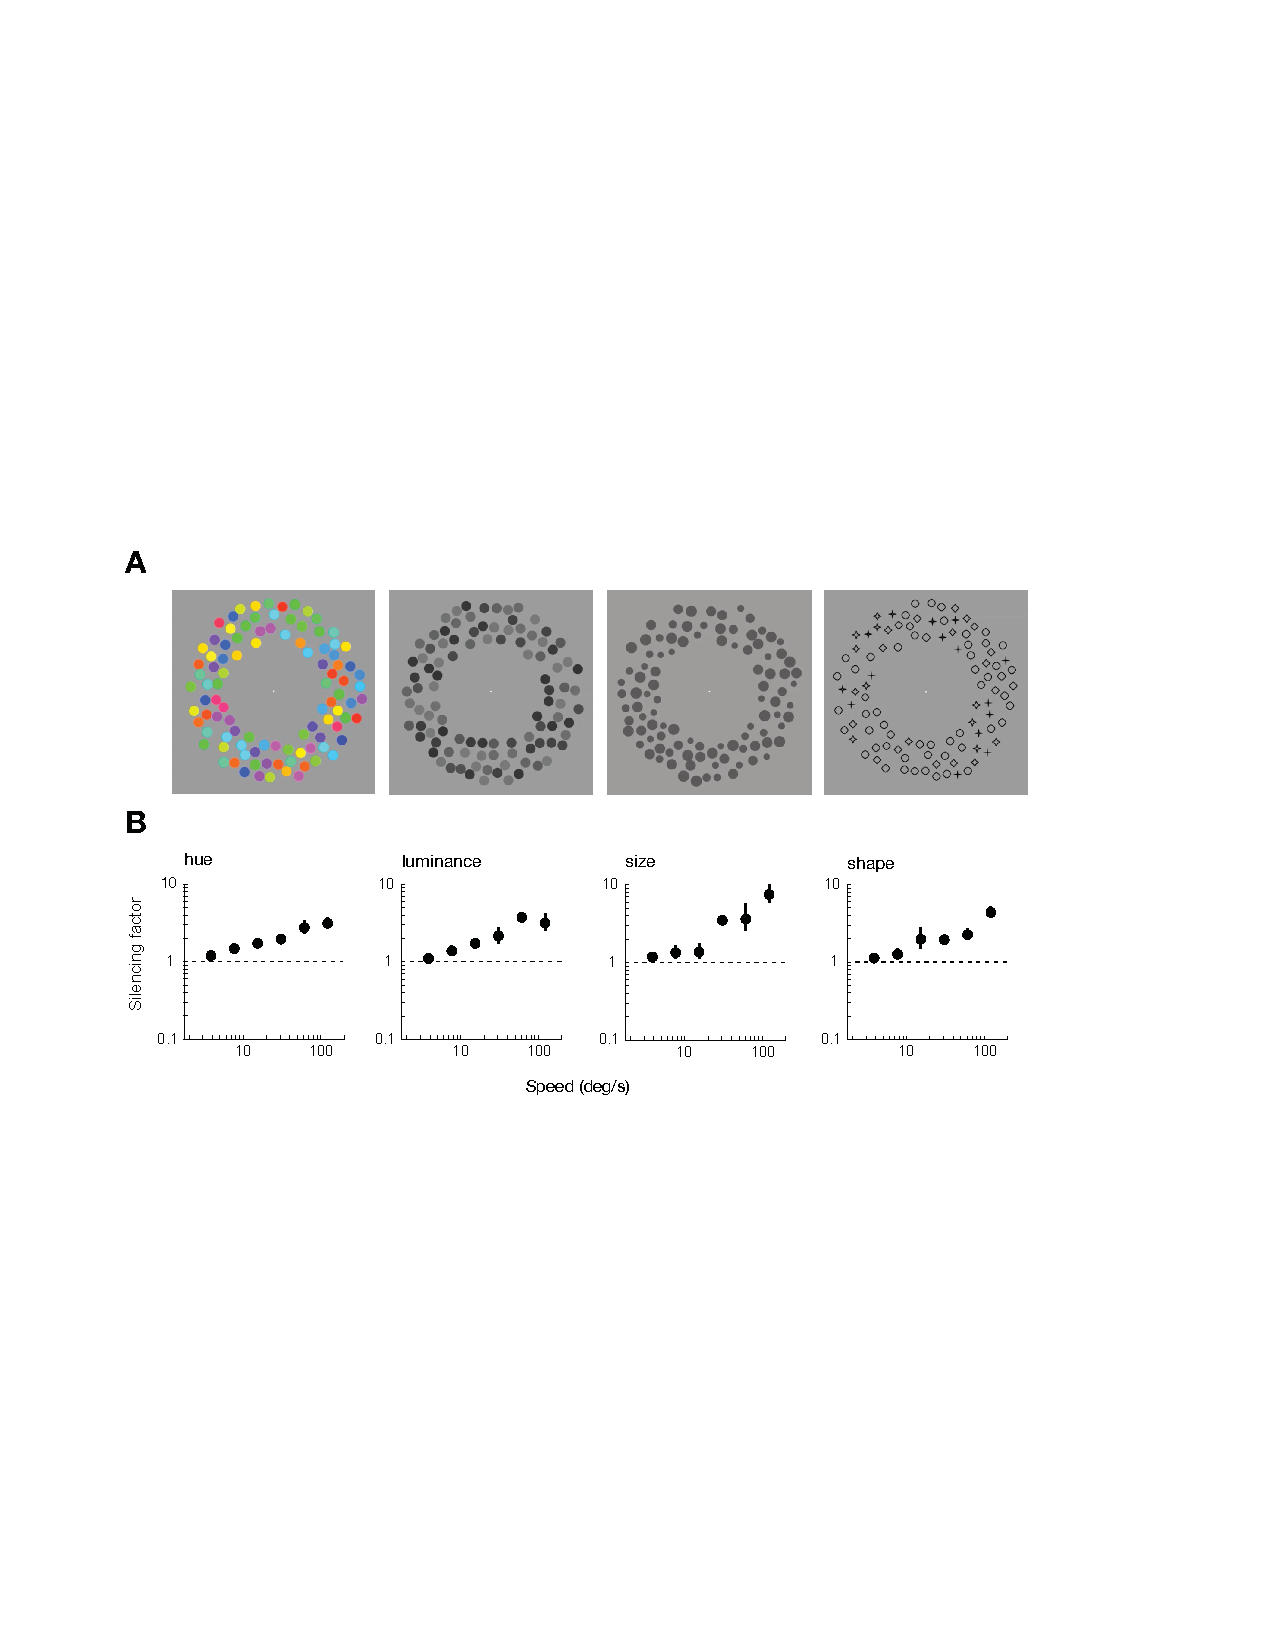
\includegraphics[width=\textwidth]{figures/fig1}
%\caption[Short figure name.]{This is a figure that floats inline and here is its caption.
%\label{fig:myInlineFigure}}
%\end{figure}

% For an example of a full page figure, see Fig.~\ref{fig:myFullPageFigure}.

%% Requires fltpage2 package
%%
% \begin{FPfigure}
% 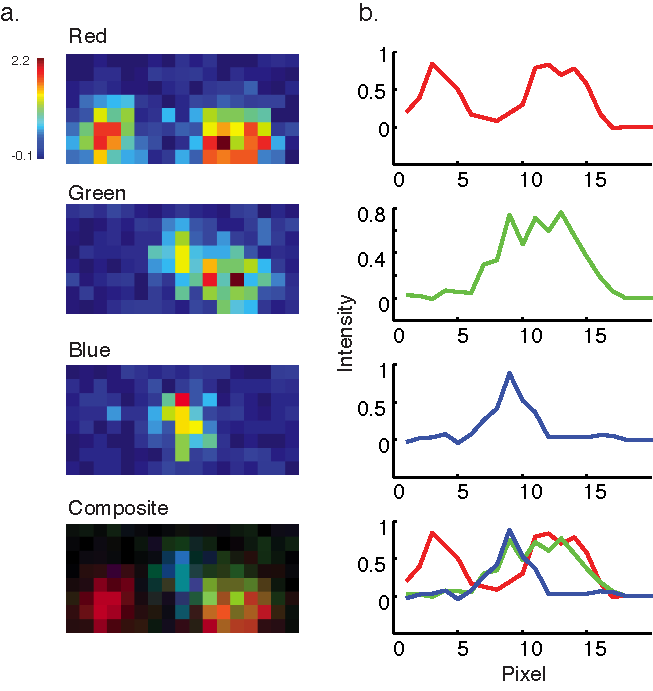
\includegraphics[width=\textwidth]{figures/fullpage}
% \caption[Short figure name.]{This is a full page figure using the FPfigure command. It takes up the whole page and the caption appears on the preceding page. Its useful for large figures. Harvard's rules about full page figures are tricky, but you don't have to worry about it because we took care of it for you. For example, the full figure is supposed to have a title in the same style as the caption but without the actual caption. The caption is supposed to appear alone on the preceding page with no other text. You do't have to worry about any of that. We have modified the fltpage package to make it work. This is a lengthy caption and it clearly would not fit on the same page as the figure. Note that you should only use the FPfigure command in instances where the figure really is too large. If the figure is small enough to fit by the caption than it does not produce the desired effect. Good luck with your thesis. I have to keep writing this to make the caption really long. LaTex is a lot of fun. You will enjoy working with it. Good luck on your post doctoral life! I am looking forward to mine. \label{fig:myFullPageFigure}}
% \end{FPfigure}
% \afterpage{\clearpage}

%\texttt{This is a line of code.}

\newthought{This chapter lays out the design and implementation} of the system used to generate optimal rule lists. 
We begin by describing each of the three main data structures used to run our algorithm--a prefix trie, a symmetry-aware map, and a queue. 
Then, we 

\section{Prefix Trie}
The prefix trie is a custom C++ class and is used as a cache to keep track of rule lists we have already evaluated. 
Each node in the trie contains the metadata associated with that corresponding rule list. 
This metadata includes bookkeeping information such as what child rule lists are feasible as well as information such as the lower bound and prediction for that rule list.
In addition to our base trie class, we implemented two different node types that we use in our algorithm.
First, we implemented a class that has an additional field that tracks the curiosity of a given prefix as defined in \ref{ch:definitions}.
Curiosity is used by our queue to determine the order that prefixes are explored.
Since the curiosity field is just a double, the memory overhead is minimal and the speed-up of using curiosity as opposed to BFS is sizable (see \ref{exp:priority}).
We also implemented a class that has an additional field keeping track of the captured vector for that prefix.
This captured vector has length $nsamples$, which means it is memory expensive.
However, using the captured vector allows us to speed up our incremental computations because we would otherwise have to recompute this vector every time we used that prefix.

\section{Queue}\label{sec:queue}
Our queue support many different types of search policies that we can use to explore the search space.
We implement a number of different scheduling schemes including BFS, DFS, various priority metrics, and a stochastic exploration process.
Due to our use of incremental computation, our queue contains pointers to leaves in the trie.
The search process involves selecting which leaf node to explore.
The stochastic exploration process bypasses the use of a queue by performing random walks on the trie until a leaf is reached.
Our other scheduling schemes use a STL C++ priority queue to hold and order all of the leaves of the trie that still need to be explored.
Our priority metrics can be ordered by curiosity, the objective of a prefix, or the lower bound of a prefix.
We find that using an exploitation strategy such as ordering by curiosity or lower bound will usually lead to a faster runtime than using BFS.

In C++ the priority queue is a wrapper container that prevents access to the container underlying the queue.
Therefore we cannot access elements in the middle of the queue, even if we have know the value that we're trying to access..
Thus, we run into a problem where we may delete something in the prefix trie that is currently in the queue but have no way to update the queue.
We deal with this by lazily marking nodes as deleted in the prefix trie without deleting the physical node until it has been popped off of the queue.
As Fig \ref{fig:queue_gc} shows, this leads to a situation where our logical queue is actually smaller than the physical queue.

\begin{figure}[t!]
\begin{center}
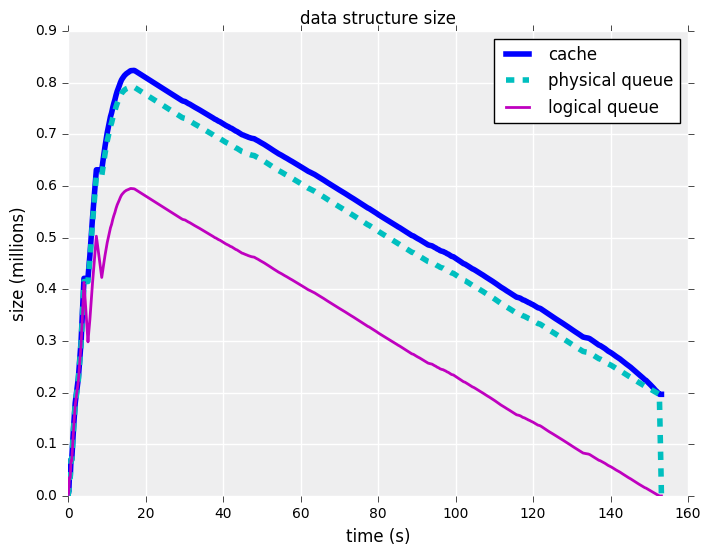
\includegraphics[width=0.65\textwidth]{figs/compas-queue-cache-size-insertions.png}
\end{center}
\caption{Size of prefix trie, logical queue, and physical queue over the execution of our algorithm. Note that the gap between the logical queue and the physical queue is due to our lazy garbage collection}
\label{fig:queue_gc}
\end{figure}

\section{Symmetry-aware map}
We implement our symmetry-aware map as an STL unordered\_map.
We use this data structure to implement the permutation bound described in \ref{def:perm-bound}.
We have two different versions of the map with different key types that allow permutations to be compared and pruned.
In both cases, the values consist of the best lower bound and the actual ordering of the rules that is best for that permutation.
In the first version, keys to the map are represented as the canonical order of the rules: i.e. the lists 3-2-1 and 2-3-1 both map to 1-2-3.
The second version has keys that represent the captured vector.
Our earlier permutation bound was based off of the fact that different permutations capture the same data, so this type of key will again be equivalent for the rule lists 3-2-1 and 2-3-1.
Representing keys with captured vectors could potentially match more permutations since two prefixes may not be permutations of each other but might capture the same data points and therefore fall under the permutation bound.
In fact, we find that this occurs only rarely, as the number of rule lists examined is only slightly less in the captured vector case.
Despite only supporting one bound, the permutation map plays a significant role in our memory usage.

\begin{figure}[t!]
\begin{center}
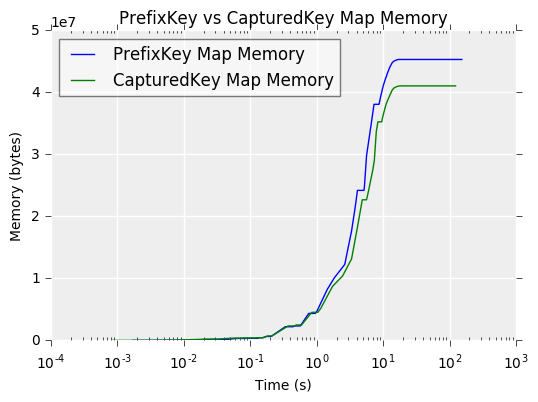
\includegraphics[width=0.7\textwidth]{figs/prefix-captured_pmap_mem.png}
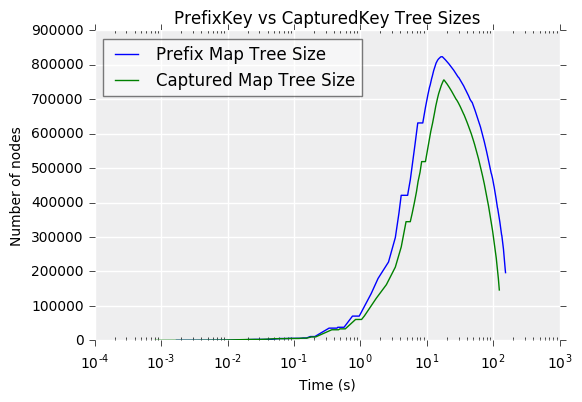
\includegraphics[width=0.7\textwidth]{figs/prefix-captured_tree_size.png}
\end{center}
\caption{This graph shows the memory usage of the map when using CapturedKeys and PrefixKeys. We see that CapturedKeys provide minimal space savings over PrefixKeys due to the slight decrease in nodes inserted into the trie.}
\label{fig:prefix-captured}
\end{figure}


\section{Incremental execution}
We detail the execution of our program below.
Our program ends when all leaves of the trie have been explored and there is nothing else in our queue.
We can also choose to not receive the full certificate of optimality by exiting execution when a certain number of rule lists are in the trie.
While there are still leaves of the trie to be explored, we use our scheduling policy to select the next rule list to evaluate.
Then, for every rule that is not already in this parent rule list, we calculate the lower bound, objective, and other metrics for the potential child rule list consisting of the new rule appended to the parent rule list.
We check the support bounds, the hierarchal objective bound, the permutation bound, and the lookahead bound.
If the child rule list has a lower bound that is better than all of these bounds, then we insert it into the permutation map, the tree, and the queue and update the minimum objective if necessary.
Otherwise, we do not insert it into any of our data structures and we continue to the next potential rule to add, having excluded a rule list from being optimal.
After evaluating all the rules we could add to our parent rule list, we return to the main loop and look at the next leaf of the trie.

\begin{algorithm}[t!]
  \caption{Branch-and-bound for learning rule lists}
\label{alg:branch-and-bound}
\begin{algorithmic}
\normalsize
\State \textbf{Output:} Outputs the best rule list and its objective\\
\State $opt \gets NULL$
\State $T \gets initializeTree()$
\State $Q \gets queue(\,[T.root()\,])$
\State $P \gets map(\{\})$
\While {$Q$ not empty}
	\State $node \gets Q$.pop(\,)
	\State $oldObj \gets T$.minObjective(\,)
	\State incremental($node, T, Q, P$) \Comment{Evaluate all of node's children}
	\If {$T$.minObjective(\,) $< oldOb$j}
		\State $opt \gets T$.bestRuleList(\,)
		\State $T$.garbageCollect(\,)
	\EndIf
\EndWhile
\State \Return $opt, T$.minObjective(\,)
\end{algorithmic}
\end{algorithm}

\begin{algorithm}[t!]
  \caption{Incremental evaluation of a prefix}
\label{alg:incremental}
\begin{algorithmic}
\normalsize
\State \textbf{Input:} Node to be evaluated~$parent$,
prefix tree~$T$,
queue~$Q$,
symmetry-aware map~$P$
\State \textbf{Output:} None---destructively updates best objective in the tree\\
\State $prefix \gets parent$.prefix(\,)
\State $t \gets c *$ nsamples \Comment{This forms the threshold for our support bounds}
\For {$rule \notin prefix$}
	\State $rlist \gets prefix$.append($rule$)
	\State $cap \gets parent\text{.notCaptured(\,)} \wedge rule$.notCaptured(\,)
	\If {$|cap| < t$} \Comment{Minimum support bound}
		\State continue
	\EndIf
	\State $capZero \gets cap \wedge T$.zeroLabel(\,) \Comment{Record how many zeros the new rule captures}
	\State $corr \gets max\{|capZero|, |cap| - |capZero|\}$
	\If {$corr < threshold$} \Comment{Minimum correct support bound}
		\State continue
	\EndIf
	\State $lb = parent.\text{bound(\,)} - parent.\text{minority(\,)} + \frac{|cap| - corr}{nsamples} + c$ \Comment{Calculate lower bound}
	\If {$lb  >= T.$minObjective(\,)} \Comment{Objective bound}
		\State continue
	\EndIf
	\State $notCap \gets parent\text{.notCaptured(\,)} \wedge \neg cap$
	\State $notCapZero \gets notCap \wedge T$.zeroLabel(\,)
	\State $defaultCorr \gets max\{|notCapZero|, |notCap - notCapZero|\}$
	\State $obj \gets lb + \frac{|notCap| - defaultCorr}{nsamples}$ \Comment{Calculate objective}
	\If {$obj < T$.minObjective(\,)} \Comment{Update minimum objective}
		\State $T.minObjective(obj)$
	\EndIf
	\If{$lb + c >= T.$minObjective(\,)} \Comment{Lookahead bound---don't add to queue if its children will all be worse than the minimum objective}
		\State continue
	\EndIf
	\State $n \gets P.insert(rlist)$ \Comment{Symmetry-aware map handles permutation bound for us}
	\If {$n$} \Comment{$n$ will be NULL if it failed the permutation bound check}
		\State $T.$insert($n$)
		\State $Q.$push($n$)
	\EndIf
\EndFor
\end{algorithmic}
\end{algorithm}

\section{Garbage Collection}
Every time we update the minimum objective, we garbage collect on the trie.
We do this by traversing from the root to all of the leaves.
Any time we encounter a node with a lower bound larger than the minimum objective, we delete its entire subtree.
In addition, if we encounter a node with no children, we prune upwards---deleting that node and recursively traversing the tree towards the root, deleting any childless nodes.
This garbage collection allows us to limit the memory usage of the trie.
In practice, though, the minimum objective is not update that often, so garbage collection is triggered only rarely.

\section{Templates vs Inheritance}
Our system has a lot of different modular parts--various priority metrics, symmetry-aware map types, and different types of information stored in trie nodes.
Since we were using C++, we took advantage of its templating system to achieve this modularity.
We believed that it would be the easiest way to switch out different components of the system, but did not think about the ramifications of this choice.
Due to code duplication, large amount of templates can lead to a much larger execution.
Indeed, with a pure templating system, our executable was 253732 bytes.

Our other alternative way to maintain modularity was to take advantage of C++'s class system and use inheritance and polymorphism.
Now, instead of having a template argument for each data structure, we can have a base data structure type and then implement each of our extensions as subclasses.
Therefore, we can write all of our functions to take the base class as arguments and then pass in the specialized subclasses based on command line arguments.
This requires the use of virtual functions, which are potentially a bit slower than regular functions because they require a vtable lookup.
With a pure inheritance framework, our executable was 171288 bytes.
However, even with the inheritance framework, the runtime of our algorithm was not significantly different from the template runtime.
Thus, since inheritance provided a much cleaner code base to work with, we decided to switch to an inheritance based framework.

\section{Memory tracking}
We track memory through the use of C++11 custom allocators.
Our allocators are simple malloc wrappers that also log which data structure the allocation is coming from--the trie, the map, or the queue.
We validated the accuracy of this memory tracking by running the program under Valgrind's massif heap profiler tool and comparing the outputs.
Our outputs matched Valgrind's to within a few hundred bytes, so we concluded that our memory tracking was successful.
The heap profiling of Valgrind has a large overhead, while our memory logging is more limited and therefore overhead is very minimal.
This allows us to write out our memory usage per data structure on a regular basis without incurring the large overhead of Valgrind.